% -----------------------------------------------------------------------------------
%                               BIBLIOGRAPHY - Insert Name of BIB File Here
% -----------------------------------------------------------------------------------
\newpage

% ---------------BIBTEX OLD-----------------------------------------------------
% \bibliographystyle{unsrt} %%%% Plain or alpha can change orders here
% \bibliography{BibFile}
% \nocite{*} %%%if you want to see all references even those note cited in the text
% -----------------------------------------------------------------------------------

\printbibliography
% -----------------------------------------------------------------------------------
%                                  APENDIX
% -----------------------------------------------------------------------------------

% \end{counted} %<<<<<<<<<<<<<<ENDS WORD COUNTER

\newpage
\section{Appendices}

\subsection{Login Guide}
\begin{itemize}

  \item Go to WordPress Login Page at ixn.host/wp-admin
  \item Use the Username: YunFu
  \item Use the Password: AppDesign

\end{itemize}

\begin{landscape}
\subsection{Competing Solutions}
  \begin{table}[H]
      \centering
      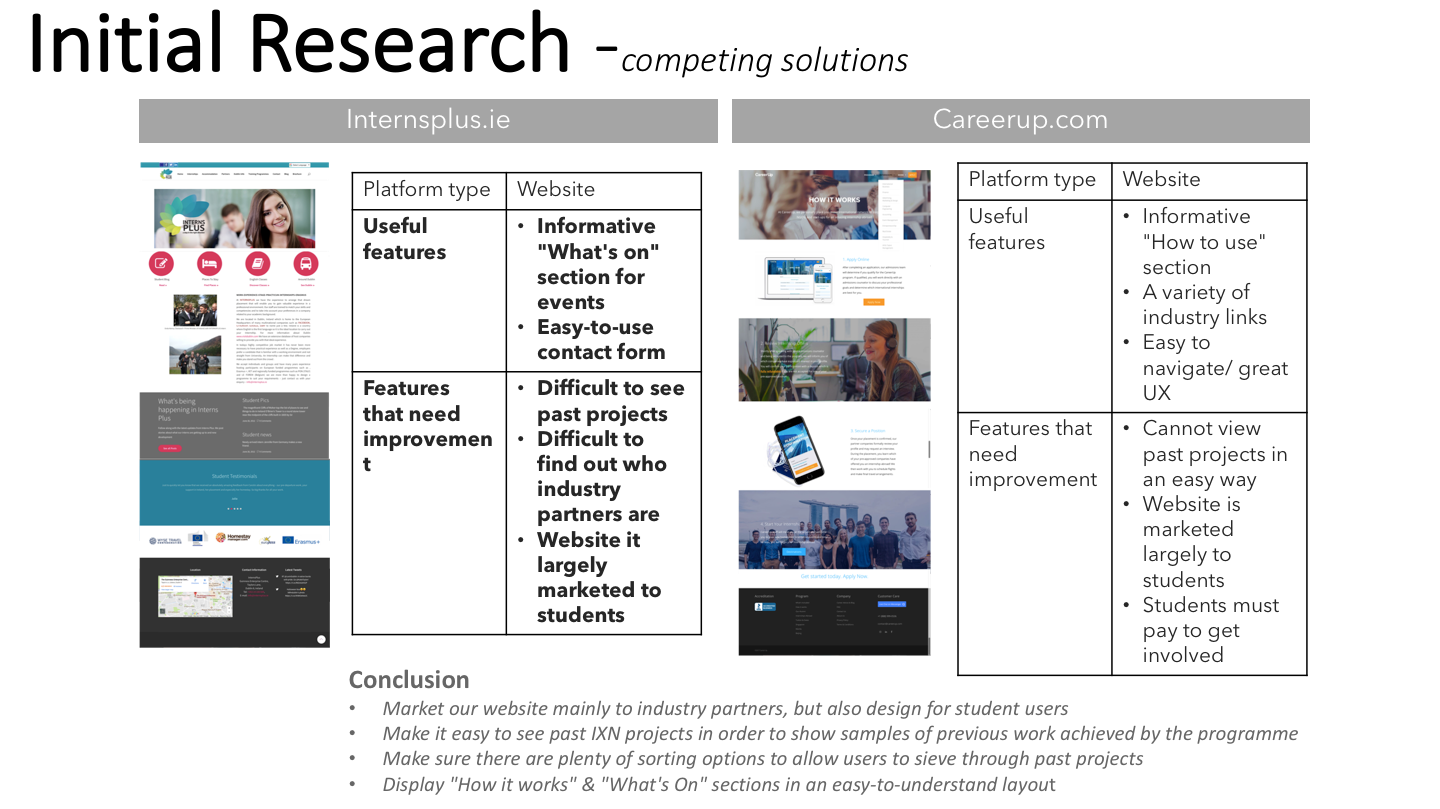
\includegraphics[trim = 0 0 0 0, clip, width=0.99\textwidth]{app5.png}
      \caption{Possible features to be implemented in the future}
 \end{table}
 \end{landscape}

 \newpage


\begin{landscape}
\subsection{Sketches}
 \begin{table}[H]
      \centering
      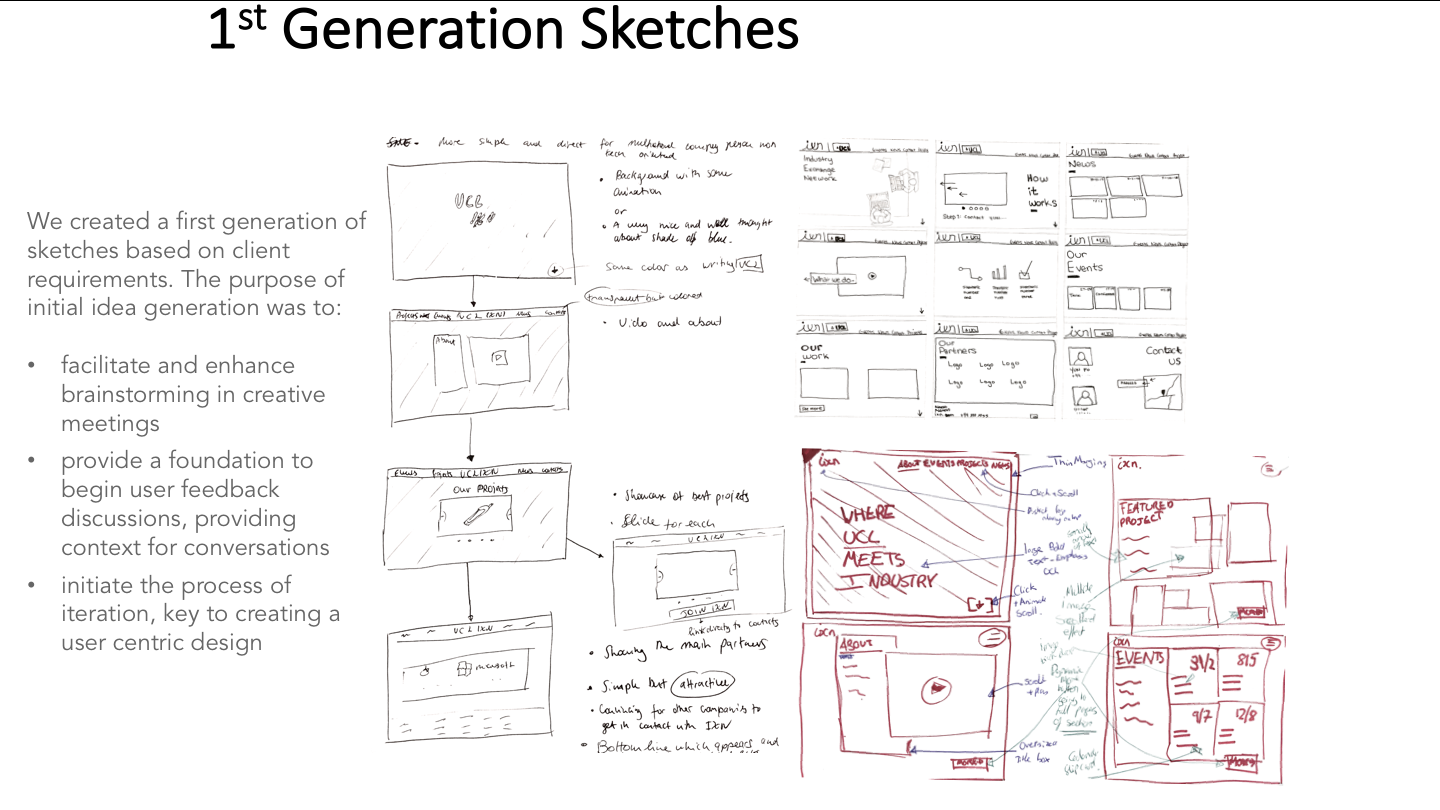
\includegraphics[trim = 0 0 0 0, clip, width=0.99\textwidth]{app4.png}
      \caption{First generation hand-drawn sketches}
 \end{table}
\end{landscape}

 \newpage

\begin{landscape}
 \begin{table}[H]
      \centering
      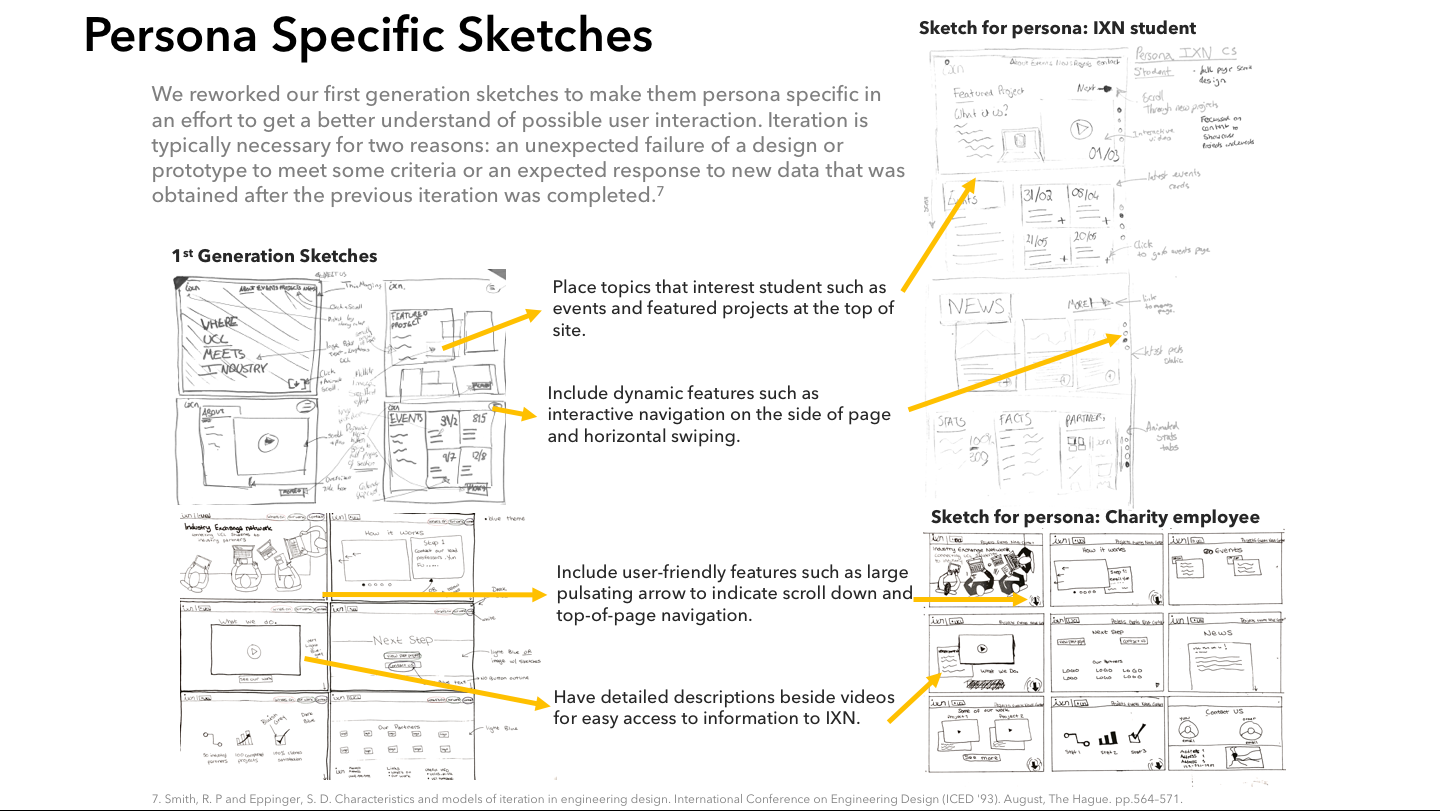
\includegraphics[trim = 0 0 0 0, clip, width=0.99\textwidth]{app3.png}
      \caption{Sketches based on researched personas}
 \end{table}
  \end{landscape}

\newpage

\begin{landscape}
\subsection{Storyboards}
 \begin{table}[H]
      \centering
      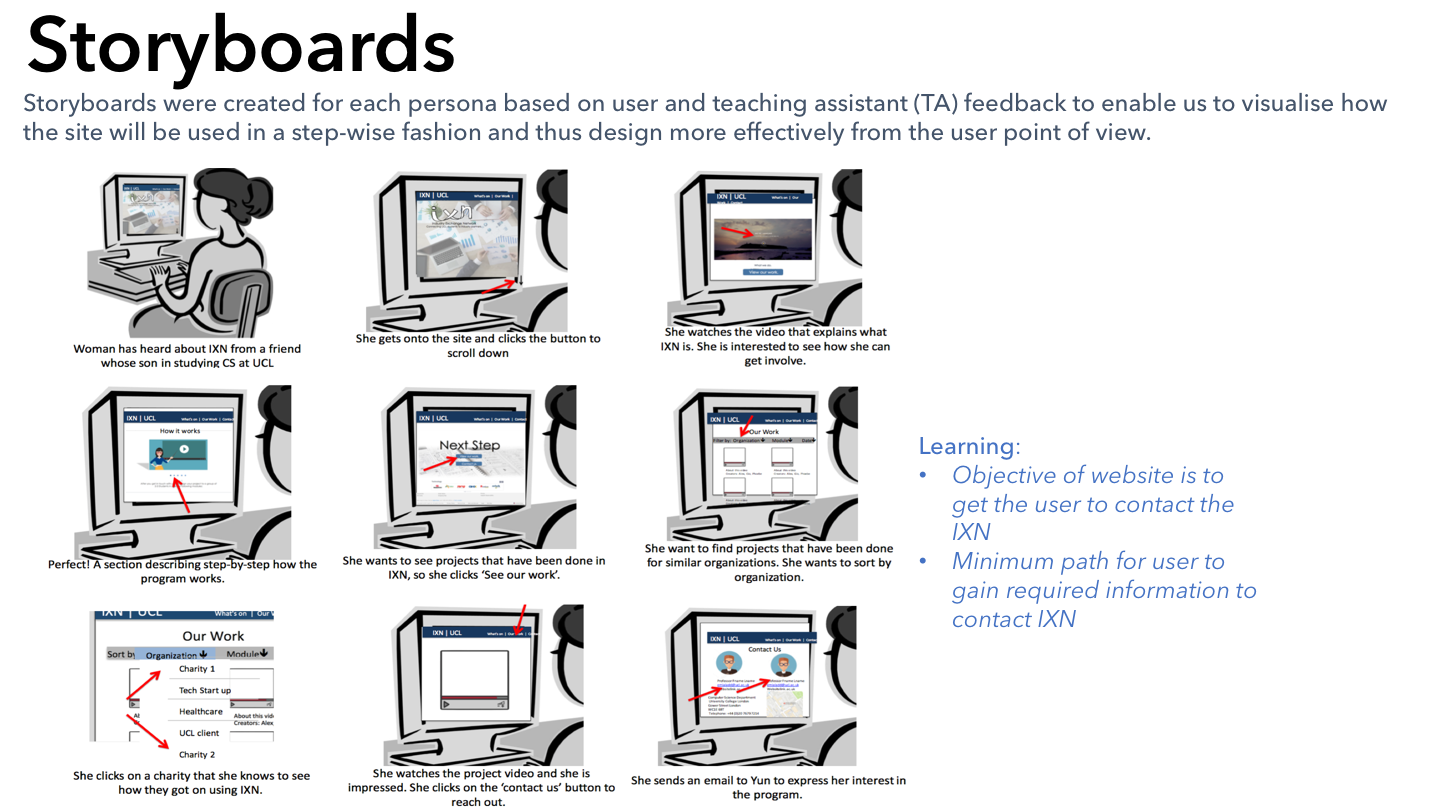
\includegraphics[trim = 0 0 0 0, clip, width=0.99\textwidth]{app2.png}
      \caption{Storyboard example describing a possible user experience.}
 \end{table}
\end{landscape}

 \newpage

\begin{landscape}
\subsection{Wire-Framing}
\begin{table}[H]
      \centering
      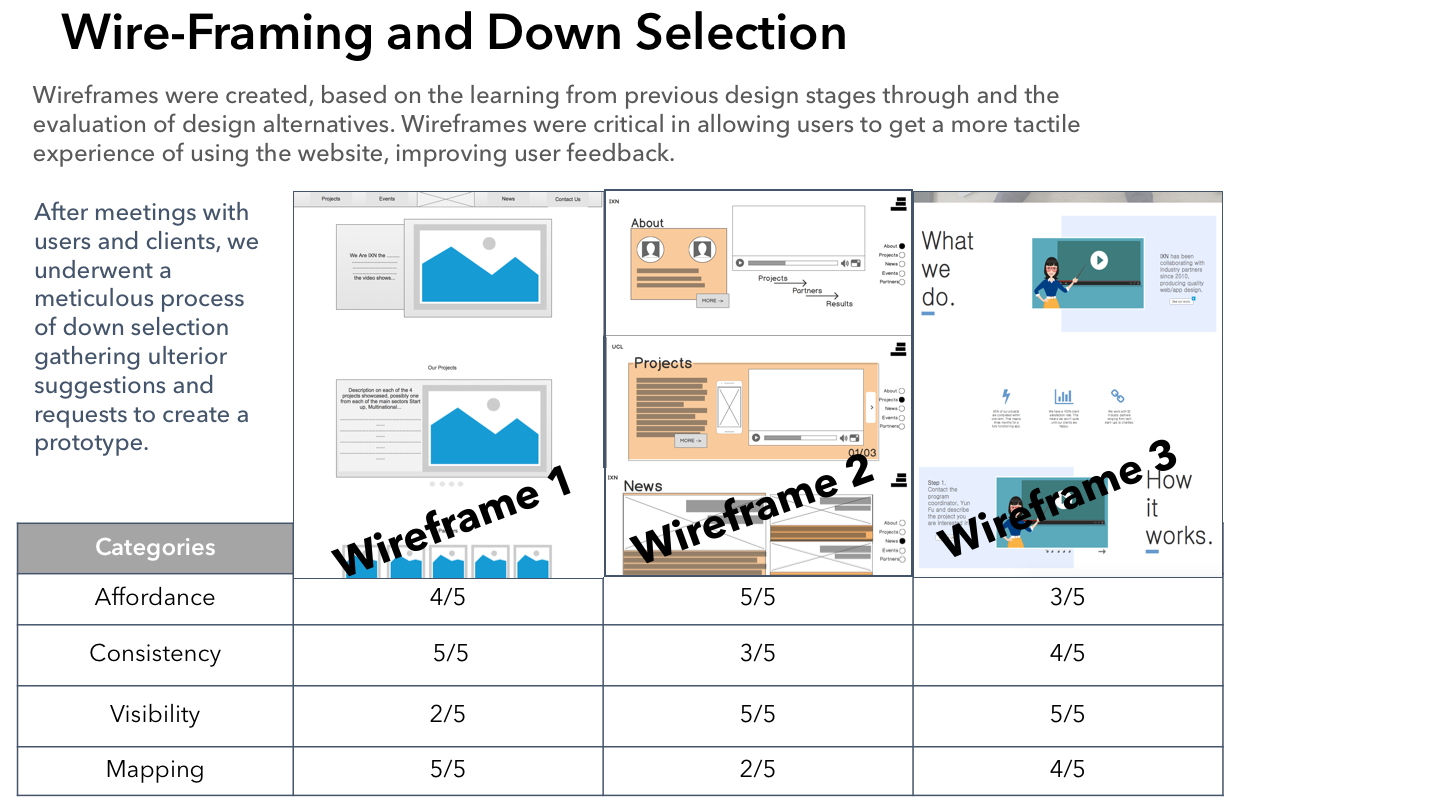
\includegraphics[trim = 0 0 0 0, clip, width=0.99\textwidth]{app1.png}
      \caption{Down selection of wire-frames.}
 \end{table}
 \end{landscape}

 \begin{landscape}
\subsection{IXN Poll}
\begin{table}[H]
      \centering
      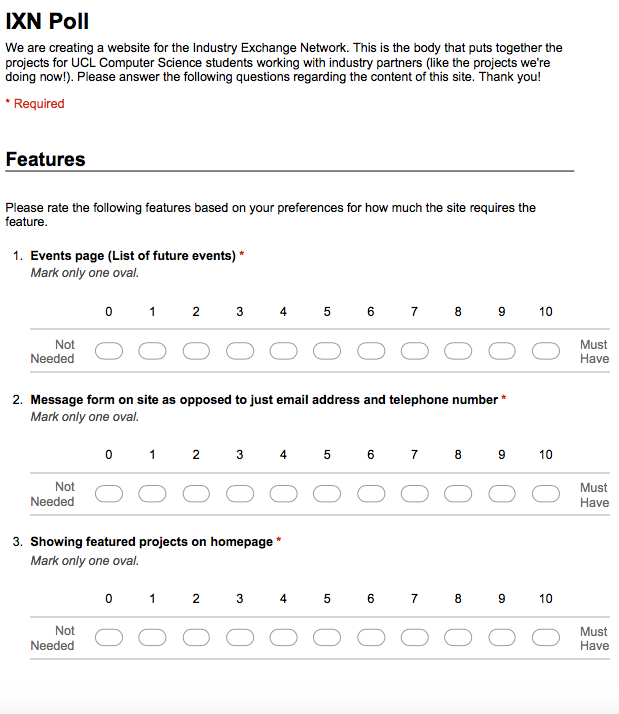
\includegraphics[trim = 0 0 0 0, clip, width=0.99\textwidth]{Poll1.png}
      \caption{IXN poll example page 1. }
 \end{table}

 \begin{table}[H]
      \centering
      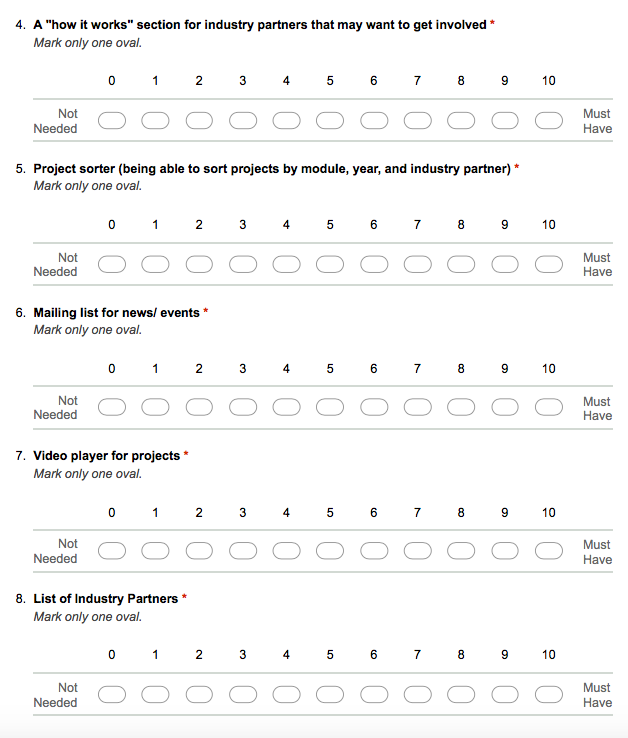
\includegraphics[trim = 0 0 0 0, clip, width=0.99\textwidth]{Poll2.png}
      \caption{IXN poll example page 2.}
 \end{table}

 \begin{table}[H]
      \centering
      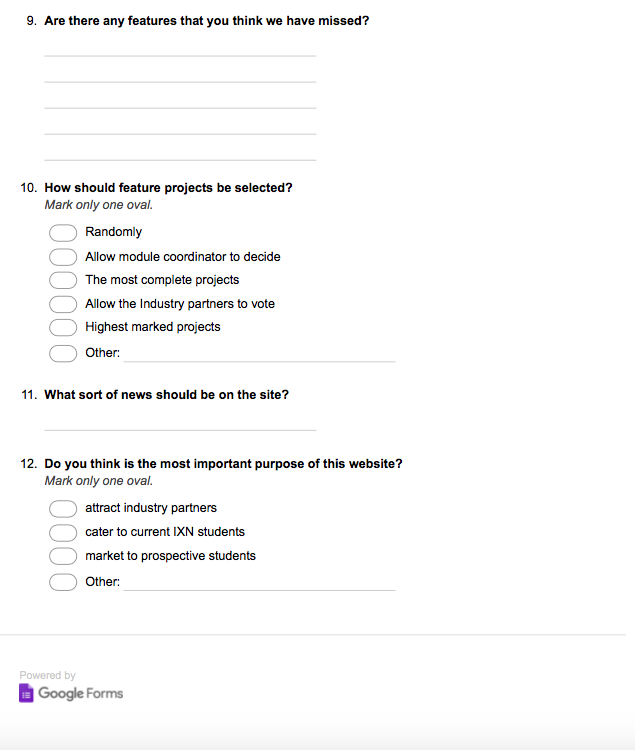
\includegraphics[trim = 0 0 0 0, clip, width=0.99\textwidth]{Poll3.png}
      \caption{IXN poll example page 3.}
 \end{table}

 \end{landscape}

 \begin{landscape}
\subsection{IXN-Poll-Results}
\begin{table}[H]
      \centering
      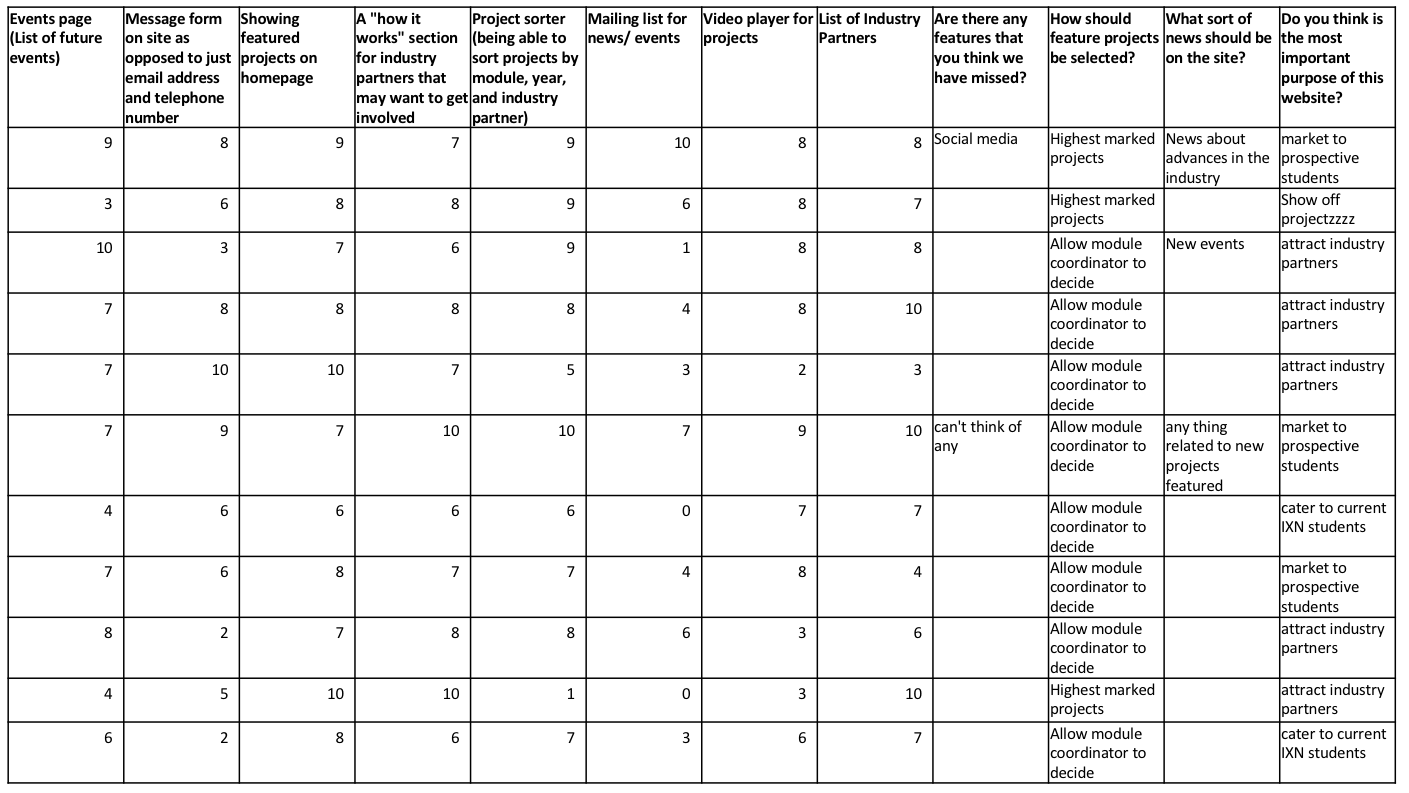
\includegraphics[trim = 0 0 0 0, clip, width=0.99\textwidth]{PollResults.png}
      \caption{Down selection of wire-frames.}
 \end{table}
 \end{landscape}

 \newpage

\begin{landscape}
\subsection{Known Bugs}
 \begin{table}[H]
      \centering
      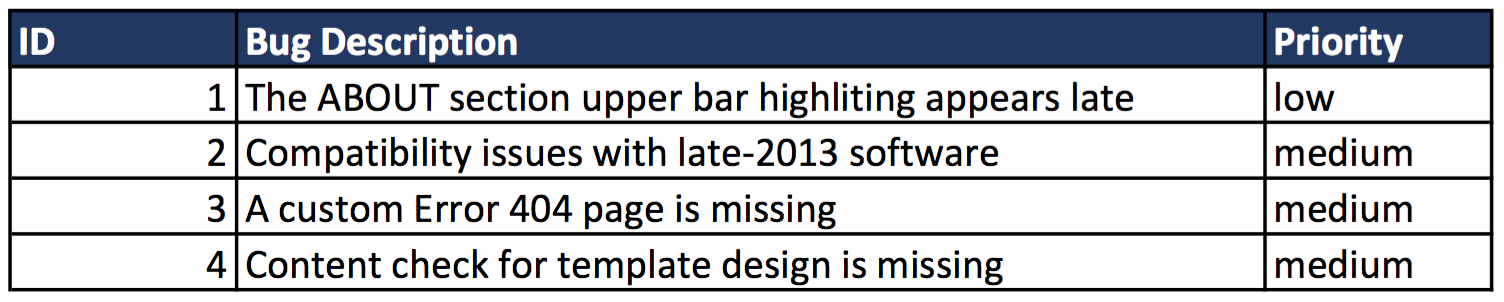
\includegraphics[trim = 0 0 0 0, clip, width=0.99\textwidth]{App7.png}
      \caption{Know bugs description and importance}
 \end{table}
\end{landscape}


\end{document}